\documentclass[tikz,border=12pt]{standalone}
\usepackage[T1]{fontenc}
\usepackage{helvet}
\renewcommand{\familydefault}{\sfdefault}
\usetikzlibrary{shapes.geometric,shapes.symbols,arrows.meta,positioning,fit,backgrounds,calc}
\hyphenpenalty=10000 \exhyphenpenalty=10000

\definecolor{ink}{HTML}{2E3440}
\definecolor{svc}{HTML}{DCE6F2}    \definecolor{svcline}{HTML}{4C6A92}
\definecolor{store}{HTML}{E5EFE1}  \definecolor{storeline}{HTML}{5B8C5A}
\definecolor{ext}{HTML}{F3E9DC}    \definecolor{extline}{HTML}{A8763E}
\definecolor{async}{HTML}{6C757D}  \definecolor{alert}{HTML}{C0392B}
\definecolor{regionfill}{HTML}{F7F9FC}

\begin{document}
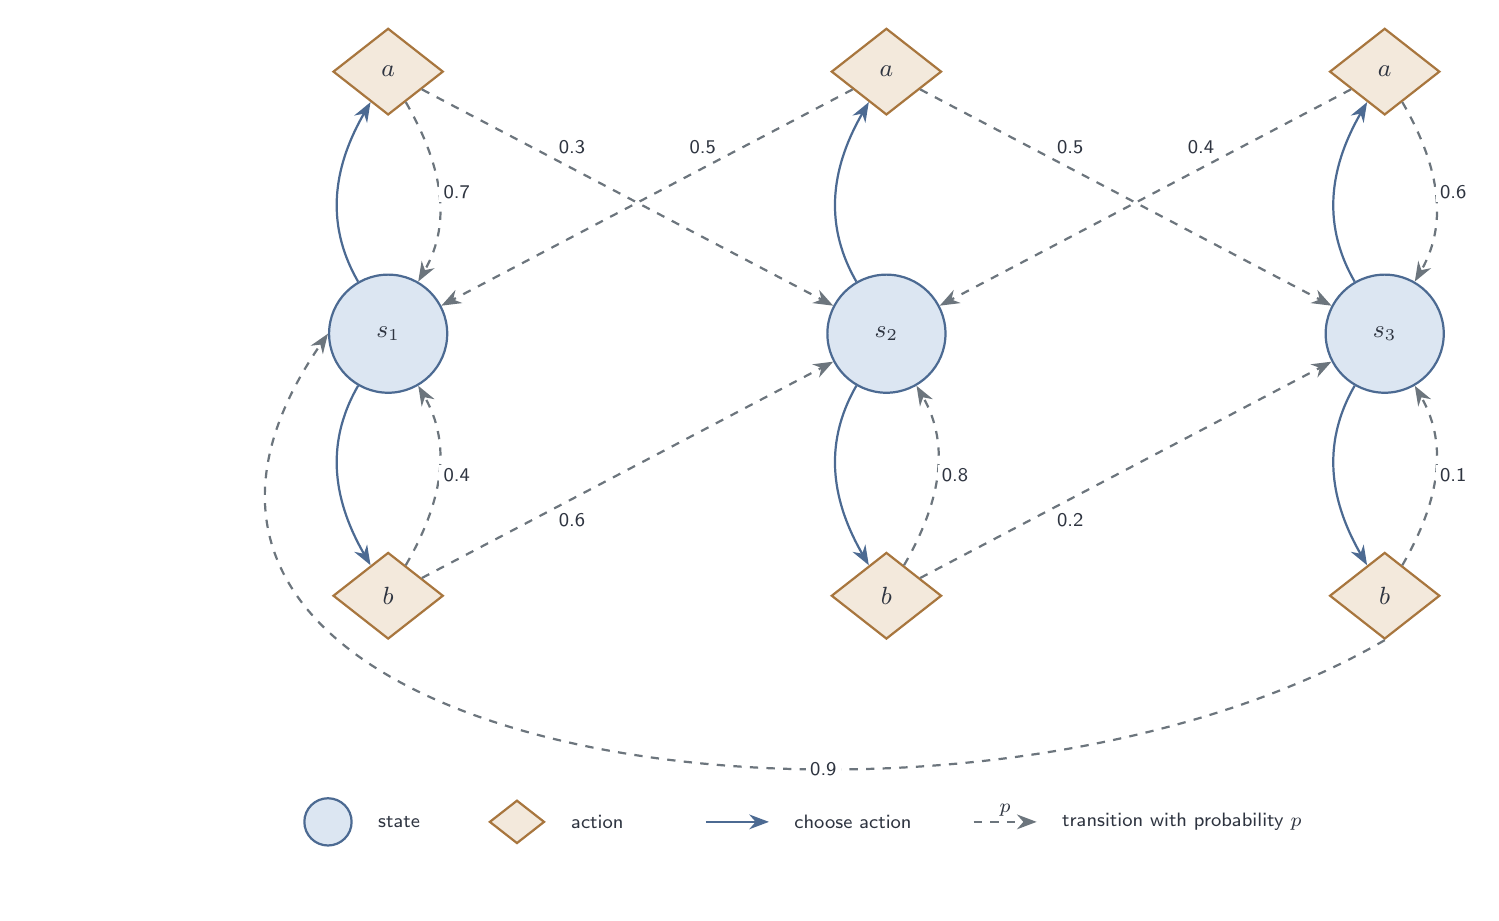
\begin{tikzpicture}[
  font=\small, color=ink, node distance=12mm and 18mm,
  state/.style={circle, draw=svcline, fill=svc, minimum size=15mm, line width=0.8pt},
  action/.style={diamond, draw=extline, fill=ext, minimum width=14mm, minimum height=11mm,
                 inner sep=1pt, line width=0.8pt},
  choose/.style={-{Stealth[length=2.5mm]}, line width=0.8pt, color=svcline},
  trans/.style={-{Stealth[length=2.5mm]}, line width=0.8pt, dashed, color=async},
  lbl/.style={font=\scriptsize, fill=white, inner sep=1.5pt, text=ink},
]
% ---- states (circles) ----
\node[state] (S1) {$s_1$};
\node[state] (S2) [right=48mm of S1] {$s_2$};
\node[state] (S3) [right=48mm of S2] {$s_3$};

% ---- actions (diamonds), one above and one below each state ----
\node[action] (a1) [above=20mm of S1] {$a$};
\node[action] (b1) [below=20mm of S1] {$b$};
\node[action] (a2) [above=20mm of S2] {$a$};
\node[action] (b2) [below=20mm of S2] {$b$};
\node[action] (a3) [above=20mm of S3] {$a$};
\node[action] (b3) [below=20mm of S3] {$b$};

% ---- state -> action (decision edges, left-hand bulge) ----
\draw[choose] (S1) to[out=120, in=-120] (a1);
\draw[choose] (S1) to[out=-120, in=120] (b1);
\draw[choose] (S2) to[out=120, in=-120] (a2);
\draw[choose] (S2) to[out=-120, in=120] (b2);
\draw[choose] (S3) to[out=120, in=-120] (a3);
\draw[choose] (S3) to[out=-120, in=120] (b3);

% ---- action -> next state (stochastic transitions with probabilities) ----
% s1, action a: 0.7 stay, 0.3 -> s2
\draw[trans] (a1) to[out=-60, in=60] node[lbl, right] {0.7} (S1);
\draw[trans] (a1) -- node[lbl, pos=0.32, above right] {0.3} (S2);
% s1, action b: 0.4 stay, 0.6 -> s2
\draw[trans] (b1) to[out=60, in=-60] node[lbl, right] {0.4} (S1);
\draw[trans] (b1) -- node[lbl, pos=0.32, below right] {0.6} (S2);
% s2, action a: 0.5 -> s1, 0.5 -> s3
\draw[trans] (a2) -- node[lbl, pos=0.32, above left] {0.5} (S1);
\draw[trans] (a2) -- node[lbl, pos=0.32, above right] {0.5} (S3);
% s2, action b: 0.8 stay, 0.2 -> s3
\draw[trans] (b2) to[out=60, in=-60] node[lbl, right] {0.8} (S2);
\draw[trans] (b2) -- node[lbl, pos=0.32, below right] {0.2} (S3);
% s3, action a: 0.4 -> s2, 0.6 stay
\draw[trans] (a3) -- node[lbl, pos=0.32, above left] {0.4} (S2);
\draw[trans] (a3) to[out=-60, in=60] node[lbl, right] {0.6} (S3);
% s3, action b: 0.9 -> s1 (routed beneath the row), 0.1 stay
\draw[trans] (b3.south) .. controls ($(b3.south)+(-55mm,-32mm)$) and ($(S1.west)+(-38mm,-55mm)$) ..
  node[lbl, pos=0.35] {0.9} (S1.west);
\draw[trans] (b3) to[out=60, in=-60] node[lbl, right] {0.1} (S3);

% ---- legend ----
\begin{scope}[shift={($(S1.west)+(0,-62mm)$)}, font=\scriptsize]
  \node[state, minimum size=6mm, font=\scriptsize] (Ls) at (0,0) {};
  \node[right=2mm of Ls, anchor=west] {state};
  \node[action, minimum width=7mm, minimum height=5.5mm, font=\scriptsize] (La) at (24mm,0) {};
  \node[right=2mm of La, anchor=west] {action};
  \draw[choose] (48mm,0) -- ++(8mm,0);
  \node[anchor=west] at (58mm,0) {choose action};
  \draw[trans] (82mm,0) -- node[lbl, above] {$p$} ++(8mm,0);
  \node[anchor=west] at (92mm,0) {transition with probability $p$};
\end{scope}
\end{tikzpicture}
\end{document}
